% Created by tikzDevice version 0.12.3.2 on 2022-01-18 14:57:38
% !TEX encoding = UTF-8 Unicode
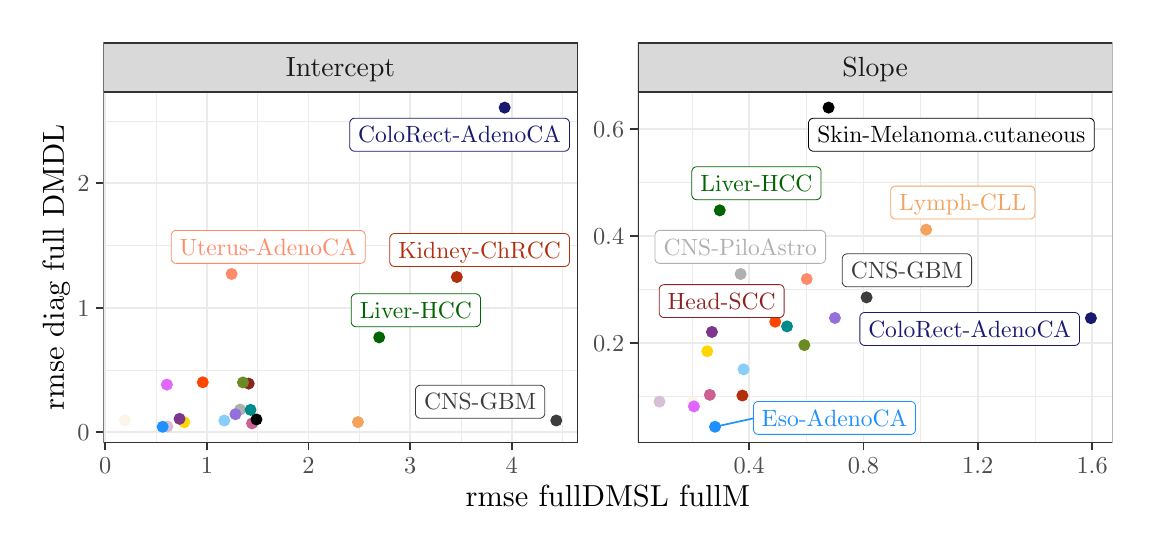
\begin{tikzpicture}[x=1pt,y=1pt]
\definecolor{fillColor}{RGB}{255,255,255}
\path[use as bounding box,fill=fillColor,fill opacity=0.00] (0,0) rectangle (397.48,180.67);
\begin{scope}
\path[clip] (  0.00,  0.00) rectangle (397.48,180.67);
\definecolor{drawColor}{RGB}{255,255,255}
\definecolor{fillColor}{RGB}{255,255,255}

\path[draw=drawColor,line width= 0.6pt,line join=round,line cap=round,fill=fillColor] (  0.00,  0.00) rectangle (397.48,180.68);
\end{scope}
\begin{scope}
\path[clip] ( 27.31, 30.69) rectangle (198.80,157.54);
\definecolor{fillColor}{RGB}{255,255,255}

\path[fill=fillColor] ( 27.31, 30.69) rectangle (198.80,157.54);
\definecolor{drawColor}{gray}{0.92}

\path[draw=drawColor,line width= 0.3pt,line join=round] ( 27.31, 56.98) --
	(198.80, 56.98);

\path[draw=drawColor,line width= 0.3pt,line join=round] ( 27.31,101.97) --
	(198.80,101.97);

\path[draw=drawColor,line width= 0.3pt,line join=round] ( 27.31,146.96) --
	(198.80,146.96);

\path[draw=drawColor,line width= 0.3pt,line join=round] ( 46.40, 30.69) --
	( 46.40,157.54);

\path[draw=drawColor,line width= 0.3pt,line join=round] ( 83.13, 30.69) --
	( 83.13,157.54);

\path[draw=drawColor,line width= 0.3pt,line join=round] (119.85, 30.69) --
	(119.85,157.54);

\path[draw=drawColor,line width= 0.3pt,line join=round] (156.58, 30.69) --
	(156.58,157.54);

\path[draw=drawColor,line width= 0.3pt,line join=round] (193.30, 30.69) --
	(193.30,157.54);

\path[draw=drawColor,line width= 0.6pt,line join=round] ( 27.31, 34.49) --
	(198.80, 34.49);

\path[draw=drawColor,line width= 0.6pt,line join=round] ( 27.31, 79.48) --
	(198.80, 79.48);

\path[draw=drawColor,line width= 0.6pt,line join=round] ( 27.31,124.46) --
	(198.80,124.46);

\path[draw=drawColor,line width= 0.6pt,line join=round] ( 28.04, 30.69) --
	( 28.04,157.54);

\path[draw=drawColor,line width= 0.6pt,line join=round] ( 64.76, 30.69) --
	( 64.76,157.54);

\path[draw=drawColor,line width= 0.6pt,line join=round] (101.49, 30.69) --
	(101.49,157.54);

\path[draw=drawColor,line width= 0.6pt,line join=round] (138.21, 30.69) --
	(138.21,157.54);

\path[draw=drawColor,line width= 0.6pt,line join=round] (174.94, 30.69) --
	(174.94,157.54);
\definecolor{drawColor}{RGB}{255,215,0}
\definecolor{fillColor}{RGB}{255,215,0}

\path[draw=drawColor,line width= 0.4pt,line join=round,line cap=round,fill=fillColor] ( 56.58, 38.09) circle (  1.96);
\definecolor{drawColor}{RGB}{205,96,144}
\definecolor{fillColor}{RGB}{205,96,144}

\path[draw=drawColor,line width= 0.4pt,line join=round,line cap=round,fill=fillColor] ( 81.07, 37.68) circle (  1.96);
\definecolor{drawColor}{gray}{0.24}
\definecolor{fillColor}{gray}{0.24}

\path[draw=drawColor,line width= 0.4pt,line join=round,line cap=round,fill=fillColor] (191.01, 38.71) circle (  1.96);
\definecolor{drawColor}{RGB}{216,191,216}
\definecolor{fillColor}{RGB}{216,191,216}

\path[draw=drawColor,line width= 0.4pt,line join=round,line cap=round,fill=fillColor] ( 50.49, 36.56) circle (  1.96);
\definecolor{drawColor}{gray}{0.69}
\definecolor{fillColor}{gray}{0.69}

\path[draw=drawColor,line width= 0.4pt,line join=round,line cap=round,fill=fillColor] ( 76.75, 42.67) circle (  1.96);
\definecolor{drawColor}{RGB}{25,25,112}
\definecolor{fillColor}{RGB}{25,25,112}

\path[draw=drawColor,line width= 0.4pt,line join=round,line cap=round,fill=fillColor] (172.35,151.78) circle (  1.96);
\definecolor{drawColor}{RGB}{30,144,255}
\definecolor{fillColor}{RGB}{30,144,255}

\path[draw=drawColor,line width= 0.4pt,line join=round,line cap=round,fill=fillColor] ( 48.77, 36.45) circle (  1.96);
\definecolor{drawColor}{RGB}{139,35,35}
\definecolor{fillColor}{RGB}{139,35,35}

\path[draw=drawColor,line width= 0.4pt,line join=round,line cap=round,fill=fillColor] ( 79.87, 52.05) circle (  1.96);
\definecolor{drawColor}{RGB}{179,47,11}
\definecolor{fillColor}{RGB}{179,47,11}

\path[draw=drawColor,line width= 0.4pt,line join=round,line cap=round,fill=fillColor] (155.07, 90.56) circle (  1.96);
\definecolor{drawColor}{RGB}{255,69,0}
\definecolor{fillColor}{RGB}{255,69,0}

\path[draw=drawColor,line width= 0.4pt,line join=round,line cap=round,fill=fillColor] ( 63.28, 52.53) circle (  1.96);
\definecolor{drawColor}{RGB}{0,100,0}
\definecolor{fillColor}{RGB}{0,100,0}

\path[draw=drawColor,line width= 0.4pt,line join=round,line cap=round,fill=fillColor] (127.02, 68.76) circle (  1.96);
\definecolor{drawColor}{RGB}{253,245,230}
\definecolor{fillColor}{RGB}{253,245,230}

\path[draw=drawColor,line width= 0.4pt,line join=round,line cap=round,fill=fillColor] ( 35.11, 38.78) circle (  1.96);
\definecolor{drawColor}{RGB}{105,139,34}
\definecolor{fillColor}{RGB}{105,139,34}

\path[draw=drawColor,line width= 0.4pt,line join=round,line cap=round,fill=fillColor] ( 77.80, 52.47) circle (  1.96);
\definecolor{drawColor}{RGB}{244,163,93}
\definecolor{fillColor}{RGB}{244,163,93}

\path[draw=drawColor,line width= 0.4pt,line join=round,line cap=round,fill=fillColor] (119.34, 38.15) circle (  1.96);
\definecolor{drawColor}{RGB}{0,139,139}
\definecolor{fillColor}{RGB}{0,139,139}

\path[draw=drawColor,line width= 0.4pt,line join=round,line cap=round,fill=fillColor] ( 80.53, 42.57) circle (  1.96);
\definecolor{drawColor}{RGB}{122,55,139}
\definecolor{fillColor}{RGB}{122,55,139}

\path[draw=drawColor,line width= 0.4pt,line join=round,line cap=round,fill=fillColor] ( 54.88, 39.32) circle (  1.96);
\definecolor{drawColor}{RGB}{224,102,255}
\definecolor{fillColor}{RGB}{224,102,255}

\path[draw=drawColor,line width= 0.4pt,line join=round,line cap=round,fill=fillColor] ( 50.30, 51.68) circle (  1.96);
\definecolor{drawColor}{RGB}{135,206,250}
\definecolor{fillColor}{RGB}{135,206,250}

\path[draw=drawColor,line width= 0.4pt,line join=round,line cap=round,fill=fillColor] ( 71.06, 38.71) circle (  1.96);
\definecolor{drawColor}{RGB}{0,0,0}
\definecolor{fillColor}{RGB}{0,0,0}

\path[draw=drawColor,line width= 0.4pt,line join=round,line cap=round,fill=fillColor] ( 82.67, 39.10) circle (  1.96);
\definecolor{drawColor}{RGB}{147,112,219}
\definecolor{fillColor}{RGB}{147,112,219}

\path[draw=drawColor,line width= 0.4pt,line join=round,line cap=round,fill=fillColor] ( 75.07, 40.98) circle (  1.96);
\definecolor{drawColor}{RGB}{255,140,105}
\definecolor{fillColor}{RGB}{255,140,105}

\path[draw=drawColor,line width= 0.4pt,line join=round,line cap=round,fill=fillColor] ( 73.69, 91.67) circle (  1.96);
\end{scope}
\begin{scope}
\path[clip] ( 27.31, 30.69) rectangle (198.80,157.54);
\definecolor{drawColor}{gray}{0.24}
\definecolor{fillColor}{RGB}{255,255,255}

\path[draw=drawColor,line width= 0.3pt,line join=round,line cap=round,fill=fillColor] (141.94, 39.55) --
	(185.06, 39.55) --
	(184.99, 39.55) --
	(185.28, 39.56) --
	(185.56, 39.62) --
	(185.84, 39.72) --
	(186.09, 39.87) --
	(186.31, 40.05) --
	(186.51, 40.27) --
	(186.66, 40.51) --
	(186.78, 40.78) --
	(186.85, 41.06) --
	(186.87, 41.35) --
	(186.87, 41.35) --
	(186.87, 49.64) --
	(186.87, 49.64) --
	(186.85, 49.93) --
	(186.78, 50.21) --
	(186.66, 50.48) --
	(186.51, 50.73) --
	(186.31, 50.94) --
	(186.09, 51.13) --
	(185.84, 51.27) --
	(185.56, 51.38) --
	(185.28, 51.44) --
	(185.06, 51.45) --
	(141.94, 51.45) --
	(142.16, 51.44) --
	(141.87, 51.45) --
	(141.58, 51.41) --
	(141.30, 51.33) --
	(141.04, 51.21) --
	(140.80, 51.04) --
	(140.59, 50.84) --
	(140.41, 50.61) --
	(140.28, 50.35) --
	(140.18, 50.07) --
	(140.14, 49.79) --
	(140.13, 49.64) --
	(140.13, 41.35) --
	(140.14, 41.50) --
	(140.14, 41.21) --
	(140.18, 40.92) --
	(140.28, 40.65) --
	(140.41, 40.39) --
	(140.59, 40.16) --
	(140.80, 39.95) --
	(141.04, 39.79) --
	(141.30, 39.66) --
	(141.58, 39.58) --
	(141.87, 39.55) --
	cycle;
\end{scope}
\begin{scope}
\path[clip] ( 27.31, 30.69) rectangle (198.80,157.54);
\definecolor{drawColor}{gray}{0.24}

\node[text=drawColor,anchor=base,inner sep=0pt, outer sep=0pt, scale=  0.85] at (163.50, 42.56) {CNS-GBM};
\definecolor{drawColor}{RGB}{25,25,112}
\definecolor{fillColor}{RGB}{255,255,255}

\path[draw=drawColor,line width= 0.3pt,line join=round,line cap=round,fill=fillColor] (118.18,136.04) --
	(193.96,136.04) --
	(193.89,136.04) --
	(194.18,136.05) --
	(194.46,136.11) --
	(194.74,136.21) --
	(194.99,136.36) --
	(195.21,136.54) --
	(195.41,136.76) --
	(195.56,137.01) --
	(195.68,137.27) --
	(195.75,137.55) --
	(195.77,137.84) --
	(195.77,137.84) --
	(195.77,146.13) --
	(195.77,146.13) --
	(195.75,146.42) --
	(195.68,146.70) --
	(195.56,146.97) --
	(195.41,147.22) --
	(195.21,147.44) --
	(194.99,147.62) --
	(194.74,147.76) --
	(194.46,147.87) --
	(194.18,147.93) --
	(193.96,147.94) --
	(118.18,147.94) --
	(118.40,147.93) --
	(118.11,147.94) --
	(117.82,147.90) --
	(117.54,147.82) --
	(117.28,147.70) --
	(117.04,147.53) --
	(116.83,147.33) --
	(116.66,147.10) --
	(116.52,146.84) --
	(116.43,146.57) --
	(116.38,146.28) --
	(116.38,146.13) --
	(116.38,137.84) --
	(116.38,137.99) --
	(116.38,137.70) --
	(116.43,137.41) --
	(116.52,137.14) --
	(116.66,136.88) --
	(116.83,136.65) --
	(117.04,136.45) --
	(117.28,136.28) --
	(117.54,136.16) --
	(117.82,136.07) --
	(118.11,136.04) --
	cycle;
\end{scope}
\begin{scope}
\path[clip] ( 27.31, 30.69) rectangle (198.80,157.54);
\definecolor{drawColor}{RGB}{25,25,112}

\node[text=drawColor,anchor=base,inner sep=0pt, outer sep=0pt, scale=  0.85] at (156.07,139.05) {ColoRect-AdenoCA};
\definecolor{drawColor}{RGB}{179,47,11}
\definecolor{fillColor}{RGB}{255,255,255}

\path[draw=drawColor,line width= 0.3pt,line join=round,line cap=round,fill=fillColor] (132.64, 94.37) --
	(193.96, 94.37) --
	(193.88, 94.38) --
	(194.17, 94.39) --
	(194.46, 94.45) --
	(194.73, 94.55) --
	(194.98, 94.69) --
	(195.21, 94.88) --
	(195.40, 95.10) --
	(195.56, 95.34) --
	(195.67, 95.61) --
	(195.74, 95.89) --
	(195.76, 96.18) --
	(195.76, 96.18) --
	(195.76,104.47) --
	(195.76,104.47) --
	(195.74,104.76) --
	(195.67,105.04) --
	(195.56,105.31) --
	(195.40,105.55) --
	(195.21,105.77) --
	(194.98,105.96) --
	(194.73,106.10) --
	(194.46,106.20) --
	(194.17,106.26) --
	(193.96,106.28) --
	(132.64,106.28) --
	(132.86,106.26) --
	(132.57,106.27) --
	(132.28,106.24) --
	(132.00,106.16) --
	(131.74,106.03) --
	(131.50,105.87) --
	(131.29,105.67) --
	(131.11,105.43) --
	(130.98,105.18) --
	(130.89,104.90) --
	(130.84,104.61) --
	(130.83,104.47) --
	(130.83, 96.18) --
	(130.84, 96.33) --
	(130.84, 96.04) --
	(130.89, 95.75) --
	(130.98, 95.47) --
	(131.11, 95.22) --
	(131.29, 94.98) --
	(131.50, 94.78) --
	(131.74, 94.62) --
	(132.00, 94.49) --
	(132.28, 94.41) --
	(132.57, 94.38) --
	cycle;
\end{scope}
\begin{scope}
\path[clip] ( 27.31, 30.69) rectangle (198.80,157.54);
\definecolor{drawColor}{RGB}{179,47,11}

\node[text=drawColor,anchor=base,inner sep=0pt, outer sep=0pt, scale=  0.85] at (163.30, 97.39) {Kidney-ChRCC};
\definecolor{drawColor}{RGB}{0,100,0}
\definecolor{fillColor}{RGB}{255,255,255}

\path[draw=drawColor,line width= 0.3pt,line join=round,line cap=round,fill=fillColor] (118.71, 72.60) --
	(161.80, 72.60) --
	(161.73, 72.60) --
	(162.02, 72.62) --
	(162.30, 72.67) --
	(162.58, 72.78) --
	(162.83, 72.92) --
	(163.05, 73.11) --
	(163.25, 73.32) --
	(163.40, 73.57) --
	(163.52, 73.84) --
	(163.59, 74.12) --
	(163.61, 74.41) --
	(163.61, 74.41) --
	(163.61, 82.70) --
	(163.61, 82.70) --
	(163.59, 82.99) --
	(163.52, 83.27) --
	(163.40, 83.54) --
	(163.25, 83.78) --
	(163.05, 84.00) --
	(162.83, 84.18) --
	(162.58, 84.33) --
	(162.30, 84.43) --
	(162.02, 84.49) --
	(161.80, 84.50) --
	(118.71, 84.50) --
	(118.93, 84.49) --
	(118.64, 84.50) --
	(118.35, 84.47) --
	(118.07, 84.39) --
	(117.81, 84.26) --
	(117.57, 84.10) --
	(117.36, 83.89) --
	(117.19, 83.66) --
	(117.05, 83.40) --
	(116.96, 83.13) --
	(116.91, 82.84) --
	(116.91, 82.70) --
	(116.91, 74.41) --
	(116.91, 74.55) --
	(116.91, 74.26) --
	(116.96, 73.98) --
	(117.05, 73.70) --
	(117.19, 73.44) --
	(117.36, 73.21) --
	(117.57, 73.01) --
	(117.81, 72.84) --
	(118.07, 72.72) --
	(118.35, 72.64) --
	(118.64, 72.60) --
	cycle;
\end{scope}
\begin{scope}
\path[clip] ( 27.31, 30.69) rectangle (198.80,157.54);
\definecolor{drawColor}{RGB}{0,100,0}

\node[text=drawColor,anchor=base,inner sep=0pt, outer sep=0pt, scale=  0.85] at (140.26, 75.61) {Liver-HCC};
\definecolor{drawColor}{RGB}{255,140,105}
\definecolor{fillColor}{RGB}{255,255,255}

\path[draw=drawColor,line width= 0.3pt,line join=round,line cap=round,fill=fillColor] ( 53.67, 95.49) --
	(120.15, 95.49) --
	(120.08, 95.50) --
	(120.37, 95.51) --
	(120.66, 95.57) --
	(120.93, 95.67) --
	(121.18, 95.81) --
	(121.40, 96.00) --
	(121.60, 96.22) --
	(121.75, 96.46) --
	(121.87, 96.73) --
	(121.94, 97.01) --
	(121.96, 97.30) --
	(121.96, 97.30) --
	(121.96,105.59) --
	(121.96,105.59) --
	(121.94,105.88) --
	(121.87,106.16) --
	(121.75,106.43) --
	(121.60,106.67) --
	(121.40,106.89) --
	(121.18,107.08) --
	(120.93,107.22) --
	(120.66,107.32) --
	(120.37,107.38) --
	(120.15,107.40) --
	( 53.67,107.40) --
	( 53.89,107.38) --
	( 53.59,107.39) --
	( 53.31,107.36) --
	( 53.03,107.28) --
	( 52.76,107.15) --
	( 52.52,106.99) --
	( 52.32,106.79) --
	( 52.14,106.55) --
	( 52.01,106.30) --
	( 51.91,106.02) --
	( 51.87,105.73) --
	( 51.86,105.59) --
	( 51.86, 97.30) --
	( 51.87, 97.45) --
	( 51.87, 97.16) --
	( 51.91, 96.87) --
	( 52.01, 96.59) --
	( 52.14, 96.34) --
	( 52.32, 96.10) --
	( 52.52, 95.90) --
	( 52.76, 95.74) --
	( 53.03, 95.61) --
	( 53.31, 95.53) --
	( 53.59, 95.50) --
	cycle;
\end{scope}
\begin{scope}
\path[clip] ( 27.31, 30.69) rectangle (198.80,157.54);
\definecolor{drawColor}{RGB}{255,140,105}

\node[text=drawColor,anchor=base,inner sep=0pt, outer sep=0pt, scale=  0.85] at ( 86.91, 98.51) {Uterus-AdenoCA};
\definecolor{drawColor}{gray}{0.20}

\path[draw=drawColor,line width= 0.6pt,line join=round,line cap=round] ( 27.31, 30.69) rectangle (198.80,157.54);
\end{scope}
\begin{scope}
\path[clip] (220.50, 30.69) rectangle (391.98,157.54);
\definecolor{fillColor}{RGB}{255,255,255}

\path[fill=fillColor] (220.50, 30.69) rectangle (391.98,157.54);
\definecolor{drawColor}{gray}{0.92}

\path[draw=drawColor,line width= 0.3pt,line join=round] (220.50, 47.35) --
	(391.98, 47.35);

\path[draw=drawColor,line width= 0.3pt,line join=round] (220.50, 86.03) --
	(391.98, 86.03);

\path[draw=drawColor,line width= 0.3pt,line join=round] (220.50,124.72) --
	(391.98,124.72);

\path[draw=drawColor,line width= 0.3pt,line join=round] (240.03, 30.69) --
	(240.03,157.54);

\path[draw=drawColor,line width= 0.3pt,line join=round] (281.35, 30.69) --
	(281.35,157.54);

\path[draw=drawColor,line width= 0.3pt,line join=round] (322.67, 30.69) --
	(322.67,157.54);

\path[draw=drawColor,line width= 0.3pt,line join=round] (363.98, 30.69) --
	(363.98,157.54);

\path[draw=drawColor,line width= 0.6pt,line join=round] (220.50, 66.69) --
	(391.98, 66.69);

\path[draw=drawColor,line width= 0.6pt,line join=round] (220.50,105.37) --
	(391.98,105.37);

\path[draw=drawColor,line width= 0.6pt,line join=round] (220.50,144.06) --
	(391.98,144.06);

\path[draw=drawColor,line width= 0.6pt,line join=round] (260.69, 30.69) --
	(260.69,157.54);

\path[draw=drawColor,line width= 0.6pt,line join=round] (302.01, 30.69) --
	(302.01,157.54);

\path[draw=drawColor,line width= 0.6pt,line join=round] (343.32, 30.69) --
	(343.32,157.54);

\path[draw=drawColor,line width= 0.6pt,line join=round] (384.64, 30.69) --
	(384.64,157.54);
\definecolor{drawColor}{RGB}{255,215,0}
\definecolor{fillColor}{RGB}{255,215,0}

\path[draw=drawColor,line width= 0.4pt,line join=round,line cap=round,fill=fillColor] (245.56, 63.75) circle (  1.96);
\definecolor{drawColor}{RGB}{205,96,144}
\definecolor{fillColor}{RGB}{205,96,144}

\path[draw=drawColor,line width= 0.4pt,line join=round,line cap=round,fill=fillColor] (246.49, 47.99) circle (  1.96);
\definecolor{drawColor}{gray}{0.24}
\definecolor{fillColor}{gray}{0.24}

\path[draw=drawColor,line width= 0.4pt,line join=round,line cap=round,fill=fillColor] (303.13, 83.21) circle (  1.96);
\definecolor{drawColor}{RGB}{216,191,216}
\definecolor{fillColor}{RGB}{216,191,216}

\path[draw=drawColor,line width= 0.4pt,line join=round,line cap=round,fill=fillColor] (228.29, 45.54) circle (  1.96);
\definecolor{drawColor}{gray}{0.69}
\definecolor{fillColor}{gray}{0.69}

\path[draw=drawColor,line width= 0.4pt,line join=round,line cap=round,fill=fillColor] (257.62, 91.66) circle (  1.96);
\definecolor{drawColor}{RGB}{25,25,112}
\definecolor{fillColor}{RGB}{25,25,112}

\path[draw=drawColor,line width= 0.4pt,line join=round,line cap=round,fill=fillColor] (384.19, 75.70) circle (  1.96);
\definecolor{drawColor}{RGB}{30,144,255}
\definecolor{fillColor}{RGB}{30,144,255}

\path[draw=drawColor,line width= 0.4pt,line join=round,line cap=round,fill=fillColor] (248.37, 36.45) circle (  1.96);
\definecolor{drawColor}{RGB}{139,35,35}
\definecolor{fillColor}{RGB}{139,35,35}

\path[draw=drawColor,line width= 0.4pt,line join=round,line cap=round,fill=fillColor] (237.54, 82.52) circle (  1.96);
\definecolor{drawColor}{RGB}{179,47,11}
\definecolor{fillColor}{RGB}{179,47,11}

\path[draw=drawColor,line width= 0.4pt,line join=round,line cap=round,fill=fillColor] (258.27, 47.74) circle (  1.96);
\definecolor{drawColor}{RGB}{255,69,0}
\definecolor{fillColor}{RGB}{255,69,0}

\path[draw=drawColor,line width= 0.4pt,line join=round,line cap=round,fill=fillColor] (270.12, 74.41) circle (  1.96);
\definecolor{drawColor}{RGB}{0,100,0}
\definecolor{fillColor}{RGB}{0,100,0}

\path[draw=drawColor,line width= 0.4pt,line join=round,line cap=round,fill=fillColor] (250.09,114.66) circle (  1.96);
\definecolor{drawColor}{RGB}{253,245,230}
\definecolor{fillColor}{RGB}{253,245,230}

\path[draw=drawColor,line width= 0.4pt,line join=round,line cap=round,fill=fillColor] (240.26, 45.34) circle (  1.96);
\definecolor{drawColor}{RGB}{105,139,34}
\definecolor{fillColor}{RGB}{105,139,34}

\path[draw=drawColor,line width= 0.4pt,line join=round,line cap=round,fill=fillColor] (280.64, 65.97) circle (  1.96);
\definecolor{drawColor}{RGB}{244,163,93}
\definecolor{fillColor}{RGB}{244,163,93}

\path[draw=drawColor,line width= 0.4pt,line join=round,line cap=round,fill=fillColor] (324.67,107.68) circle (  1.96);
\definecolor{drawColor}{RGB}{0,139,139}
\definecolor{fillColor}{RGB}{0,139,139}

\path[draw=drawColor,line width= 0.4pt,line join=round,line cap=round,fill=fillColor] (274.39, 72.73) circle (  1.96);
\definecolor{drawColor}{RGB}{122,55,139}
\definecolor{fillColor}{RGB}{122,55,139}

\path[draw=drawColor,line width= 0.4pt,line join=round,line cap=round,fill=fillColor] (247.25, 70.71) circle (  1.96);
\definecolor{drawColor}{RGB}{224,102,255}
\definecolor{fillColor}{RGB}{224,102,255}

\path[draw=drawColor,line width= 0.4pt,line join=round,line cap=round,fill=fillColor] (240.74, 43.81) circle (  1.96);
\definecolor{drawColor}{RGB}{135,206,250}
\definecolor{fillColor}{RGB}{135,206,250}

\path[draw=drawColor,line width= 0.4pt,line join=round,line cap=round,fill=fillColor] (258.69, 57.21) circle (  1.96);
\definecolor{drawColor}{RGB}{0,0,0}
\definecolor{fillColor}{RGB}{0,0,0}

\path[draw=drawColor,line width= 0.4pt,line join=round,line cap=round,fill=fillColor] (289.40,151.78) circle (  1.96);
\definecolor{drawColor}{RGB}{147,112,219}
\definecolor{fillColor}{RGB}{147,112,219}

\path[draw=drawColor,line width= 0.4pt,line join=round,line cap=round,fill=fillColor] (291.70, 75.77) circle (  1.96);
\definecolor{drawColor}{RGB}{255,140,105}
\definecolor{fillColor}{RGB}{255,140,105}

\path[draw=drawColor,line width= 0.4pt,line join=round,line cap=round,fill=fillColor] (281.51, 89.85) circle (  1.96);
\end{scope}
\begin{scope}
\path[clip] (220.50, 30.69) rectangle (391.98,157.54);
\definecolor{drawColor}{RGB}{30,144,255}

\path[draw=drawColor,line width= 0.6pt,line join=round,line cap=round] (262.26, 39.50) -- (249.44, 36.69);
\definecolor{drawColor}{gray}{0.24}
\definecolor{fillColor}{RGB}{255,255,255}

\path[draw=drawColor,line width= 0.3pt,line join=round,line cap=round,fill=fillColor] (296.15, 87.05) --
	(339.27, 87.05) --
	(339.20, 87.05) --
	(339.49, 87.06) --
	(339.77, 87.12) --
	(340.05, 87.22) --
	(340.30, 87.37) --
	(340.52, 87.55) --
	(340.72, 87.77) --
	(340.87, 88.02) --
	(340.99, 88.28) --
	(341.05, 88.57) --
	(341.08, 88.86) --
	(341.08, 88.86) --
	(341.08, 97.14) --
	(341.08, 97.14) --
	(341.05, 97.43) --
	(340.99, 97.72) --
	(340.87, 97.98) --
	(340.72, 98.23) --
	(340.52, 98.45) --
	(340.30, 98.63) --
	(340.05, 98.78) --
	(339.77, 98.88) --
	(339.49, 98.94) --
	(339.27, 98.95) --
	(296.15, 98.95) --
	(296.37, 98.94) --
	(296.08, 98.95) --
	(295.79, 98.91) --
	(295.51, 98.83) --
	(295.24, 98.71) --
	(295.01, 98.54) --
	(294.80, 98.34) --
	(294.62, 98.11) --
	(294.49, 97.85) --
	(294.39, 97.58) --
	(294.35, 97.29) --
	(294.34, 97.14) --
	(294.34, 88.86) --
	(294.35, 89.00) --
	(294.35, 88.71) --
	(294.39, 88.42) --
	(294.49, 88.15) --
	(294.62, 87.89) --
	(294.80, 87.66) --
	(295.01, 87.46) --
	(295.24, 87.29) --
	(295.51, 87.17) --
	(295.79, 87.09) --
	(296.08, 87.05) --
	cycle;
\end{scope}
\begin{scope}
\path[clip] (220.50, 30.69) rectangle (391.98,157.54);
\definecolor{drawColor}{gray}{0.24}

\node[text=drawColor,anchor=base,inner sep=0pt, outer sep=0pt, scale=  0.85] at (317.71, 90.06) {CNS-GBM};
\definecolor{drawColor}{gray}{0.69}
\definecolor{fillColor}{RGB}{255,255,255}

\path[draw=drawColor,line width= 0.3pt,line join=round,line cap=round,fill=fillColor] (228.46, 95.51) --
	(286.53, 95.51) --
	(286.46, 95.51) --
	(286.75, 95.52) --
	(287.04, 95.58) --
	(287.31, 95.68) --
	(287.56, 95.83) --
	(287.78, 96.01) --
	(287.98, 96.23) --
	(288.13, 96.47) --
	(288.25, 96.74) --
	(288.32, 97.02) --
	(288.34, 97.31) --
	(288.34, 97.31) --
	(288.34,105.60) --
	(288.34,105.60) --
	(288.32,105.89) --
	(288.25,106.17) --
	(288.13,106.44) --
	(287.98,106.69) --
	(287.78,106.90) --
	(287.56,107.09) --
	(287.31,107.23) --
	(287.04,107.34) --
	(286.75,107.39) --
	(286.53,107.41) --
	(228.46,107.41) --
	(228.68,107.39) --
	(228.39,107.41) --
	(228.10,107.37) --
	(227.82,107.29) --
	(227.56,107.17) --
	(227.32,107.00) --
	(227.11,106.80) --
	(226.94,106.57) --
	(226.80,106.31) --
	(226.71,106.03) --
	(226.66,105.75) --
	(226.66,105.60) --
	(226.66, 97.31) --
	(226.66, 97.46) --
	(226.66, 97.17) --
	(226.71, 96.88) --
	(226.80, 96.60) --
	(226.94, 96.35) --
	(227.11, 96.11) --
	(227.32, 95.91) --
	(227.56, 95.75) --
	(227.82, 95.62) --
	(228.10, 95.54) --
	(228.39, 95.51) --
	cycle;
\end{scope}
\begin{scope}
\path[clip] (220.50, 30.69) rectangle (391.98,157.54);
\definecolor{drawColor}{gray}{0.69}

\node[text=drawColor,anchor=base,inner sep=0pt, outer sep=0pt, scale=  0.85] at (257.50, 98.52) {CNS-PiloAstro};
\definecolor{drawColor}{RGB}{25,25,112}
\definecolor{fillColor}{RGB}{255,255,255}

\path[draw=drawColor,line width= 0.3pt,line join=round,line cap=round,fill=fillColor] (302.51, 65.85) --
	(378.29, 65.85) --
	(378.21, 65.85) --
	(378.51, 65.86) --
	(378.79, 65.92) --
	(379.06, 66.02) --
	(379.31, 66.17) --
	(379.54, 66.35) --
	(379.73, 66.57) --
	(379.89, 66.81) --
	(380.00, 67.08) --
	(380.07, 67.36) --
	(380.09, 67.65) --
	(380.09, 67.65) --
	(380.09, 75.94) --
	(380.09, 75.94) --
	(380.07, 76.23) --
	(380.00, 76.51) --
	(379.89, 76.78) --
	(379.73, 77.03) --
	(379.54, 77.25) --
	(379.31, 77.43) --
	(379.06, 77.57) --
	(378.79, 77.68) --
	(378.51, 77.74) --
	(378.29, 77.75) --
	(302.51, 77.75) --
	(302.73, 77.74) --
	(302.44, 77.75) --
	(302.15, 77.71) --
	(301.87, 77.63) --
	(301.61, 77.51) --
	(301.37, 77.34) --
	(301.16, 77.14) --
	(300.98, 76.91) --
	(300.85, 76.65) --
	(300.76, 76.37) --
	(300.71, 76.09) --
	(300.70, 75.94) --
	(300.70, 67.65) --
	(300.71, 67.80) --
	(300.71, 67.51) --
	(300.76, 67.22) --
	(300.85, 66.95) --
	(300.98, 66.69) --
	(301.16, 66.46) --
	(301.37, 66.26) --
	(301.61, 66.09) --
	(301.87, 65.97) --
	(302.15, 65.88) --
	(302.44, 65.85) --
	cycle;
\end{scope}
\begin{scope}
\path[clip] (220.50, 30.69) rectangle (391.98,157.54);
\definecolor{drawColor}{RGB}{25,25,112}

\node[text=drawColor,anchor=base,inner sep=0pt, outer sep=0pt, scale=  0.85] at (340.40, 68.86) {ColoRect-AdenoCA};
\definecolor{drawColor}{RGB}{30,144,255}
\definecolor{fillColor}{RGB}{255,255,255}

\path[draw=drawColor,line width= 0.3pt,line join=round,line cap=round,fill=fillColor] (264.07, 33.70) --
	(319.03, 33.70) --
	(318.96, 33.70) --
	(319.25, 33.71) --
	(319.54, 33.77) --
	(319.81, 33.87) --
	(320.06, 34.02) --
	(320.29, 34.20) --
	(320.48, 34.42) --
	(320.63, 34.66) --
	(320.75, 34.93) --
	(320.82, 35.21) --
	(320.84, 35.50) --
	(320.84, 35.50) --
	(320.84, 43.79) --
	(320.84, 43.79) --
	(320.82, 44.08) --
	(320.75, 44.36) --
	(320.63, 44.63) --
	(320.48, 44.88) --
	(320.29, 45.09) --
	(320.06, 45.28) --
	(319.81, 45.42) --
	(319.54, 45.53) --
	(319.25, 45.59) --
	(319.03, 45.60) --
	(264.07, 45.60) --
	(264.29, 45.59) --
	(264.00, 45.60) --
	(263.71, 45.56) --
	(263.43, 45.48) --
	(263.17, 45.36) --
	(262.93, 45.19) --
	(262.72, 44.99) --
	(262.54, 44.76) --
	(262.41, 44.50) --
	(262.32, 44.22) --
	(262.27, 43.94) --
	(262.26, 43.79) --
	(262.26, 35.50) --
	(262.27, 35.65) --
	(262.27, 35.36) --
	(262.32, 35.07) --
	(262.41, 34.80) --
	(262.54, 34.54) --
	(262.72, 34.31) --
	(262.93, 34.10) --
	(263.17, 33.94) --
	(263.43, 33.81) --
	(263.71, 33.73) --
	(264.00, 33.70) --
	cycle;
\end{scope}
\begin{scope}
\path[clip] (220.50, 30.69) rectangle (391.98,157.54);
\definecolor{drawColor}{RGB}{30,144,255}

\node[text=drawColor,anchor=base,inner sep=0pt, outer sep=0pt, scale=  0.85] at (291.55, 36.71) {Eso-AdenoCA};
\definecolor{drawColor}{RGB}{139,35,35}
\definecolor{fillColor}{RGB}{255,255,255}

\path[draw=drawColor,line width= 0.3pt,line join=round,line cap=round,fill=fillColor] (230.01, 75.92) --
	(271.53, 75.92) --
	(271.46, 75.92) --
	(271.75, 75.93) --
	(272.03, 75.99) --
	(272.31, 76.09) --
	(272.56, 76.23) --
	(272.78, 76.42) --
	(272.98, 76.64) --
	(273.13, 76.88) --
	(273.24, 77.15) --
	(273.31, 77.43) --
	(273.34, 77.72) --
	(273.34, 77.72) --
	(273.34, 86.01) --
	(273.34, 86.01) --
	(273.31, 86.30) --
	(273.24, 86.58) --
	(273.13, 86.85) --
	(272.98, 87.10) --
	(272.78, 87.31) --
	(272.56, 87.50) --
	(272.31, 87.64) --
	(272.03, 87.75) --
	(271.75, 87.80) --
	(271.53, 87.82) --
	(230.01, 87.82) --
	(230.23, 87.80) --
	(229.94, 87.82) --
	(229.65, 87.78) --
	(229.37, 87.70) --
	(229.10, 87.57) --
	(228.87, 87.41) --
	(228.66, 87.21) --
	(228.48, 86.98) --
	(228.35, 86.72) --
	(228.25, 86.44) --
	(228.21, 86.16) --
	(228.20, 86.01) --
	(228.20, 77.72) --
	(228.21, 77.87) --
	(228.21, 77.58) --
	(228.25, 77.29) --
	(228.35, 77.01) --
	(228.48, 76.76) --
	(228.66, 76.52) --
	(228.87, 76.32) --
	(229.10, 76.16) --
	(229.37, 76.03) --
	(229.65, 75.95) --
	(229.94, 75.92) --
	cycle;
\end{scope}
\begin{scope}
\path[clip] (220.50, 30.69) rectangle (391.98,157.54);
\definecolor{drawColor}{RGB}{139,35,35}

\node[text=drawColor,anchor=base,inner sep=0pt, outer sep=0pt, scale=  0.85] at (250.77, 78.93) {Head-SCC};
\definecolor{drawColor}{RGB}{0,100,0}
\definecolor{fillColor}{RGB}{255,255,255}

\path[draw=drawColor,line width= 0.3pt,line join=round,line cap=round,fill=fillColor] (241.79,118.50) --
	(284.88,118.50) --
	(284.80,118.51) --
	(285.10,118.52) --
	(285.38,118.58) --
	(285.65,118.68) --
	(285.90,118.82) --
	(286.13,119.01) --
	(286.32,119.23) --
	(286.48,119.47) --
	(286.59,119.74) --
	(286.66,120.02) --
	(286.68,120.31) --
	(286.68,120.31) --
	(286.68,128.60) --
	(286.68,128.60) --
	(286.66,128.89) --
	(286.59,129.17) --
	(286.48,129.44) --
	(286.32,129.68) --
	(286.13,129.90) --
	(285.90,130.09) --
	(285.65,130.23) --
	(285.38,130.33) --
	(285.10,130.39) --
	(284.88,130.41) --
	(241.79,130.41) --
	(242.01,130.39) --
	(241.72,130.40) --
	(241.43,130.37) --
	(241.15,130.29) --
	(240.89,130.16) --
	(240.65,130.00) --
	(240.44,129.80) --
	(240.26,129.56) --
	(240.13,129.31) --
	(240.04,129.03) --
	(239.99,128.74) --
	(239.98,128.60) --
	(239.98,120.31) --
	(239.99,120.46) --
	(239.99,120.17) --
	(240.04,119.88) --
	(240.13,119.60) --
	(240.26,119.35) --
	(240.44,119.11) --
	(240.65,118.91) --
	(240.89,118.75) --
	(241.15,118.62) --
	(241.43,118.54) --
	(241.72,118.51) --
	cycle;
\end{scope}
\begin{scope}
\path[clip] (220.50, 30.69) rectangle (391.98,157.54);
\definecolor{drawColor}{RGB}{0,100,0}

\node[text=drawColor,anchor=base,inner sep=0pt, outer sep=0pt, scale=  0.85] at (263.33,121.52) {Liver-HCC};
\definecolor{drawColor}{RGB}{244,163,93}
\definecolor{fillColor}{RGB}{255,255,255}

\path[draw=drawColor,line width= 0.3pt,line join=round,line cap=round,fill=fillColor] (313.64,111.52) --
	(362.16,111.52) --
	(362.09,111.52) --
	(362.38,111.54) --
	(362.66,111.59) --
	(362.93,111.70) --
	(363.19,111.84) --
	(363.41,112.03) --
	(363.60,112.24) --
	(363.76,112.49) --
	(363.87,112.76) --
	(363.94,113.04) --
	(363.97,113.33) --
	(363.97,113.33) --
	(363.97,121.62) --
	(363.97,121.62) --
	(363.94,121.91) --
	(363.87,122.19) --
	(363.76,122.46) --
	(363.60,122.70) --
	(363.41,122.92) --
	(363.19,123.10) --
	(362.93,123.25) --
	(362.66,123.35) --
	(362.38,123.41) --
	(362.16,123.42) --
	(313.64,123.42) --
	(313.86,123.41) --
	(313.57,123.42) --
	(313.28,123.39) --
	(313.00,123.31) --
	(312.74,123.18) --
	(312.50,123.02) --
	(312.29,122.81) --
	(312.12,122.58) --
	(311.98,122.32) --
	(311.89,122.05) --
	(311.84,121.76) --
	(311.84,121.62) --
	(311.84,113.33) --
	(311.84,113.47) --
	(311.84,113.18) --
	(311.89,112.90) --
	(311.98,112.62) --
	(312.12,112.36) --
	(312.29,112.13) --
	(312.50,111.93) --
	(312.74,111.76) --
	(313.00,111.64) --
	(313.28,111.56) --
	(313.57,111.52) --
	cycle;
\end{scope}
\begin{scope}
\path[clip] (220.50, 30.69) rectangle (391.98,157.54);
\definecolor{drawColor}{RGB}{244,163,93}

\node[text=drawColor,anchor=base,inner sep=0pt, outer sep=0pt, scale=  0.85] at (337.90,114.53) {Lymph-CLL};
\definecolor{drawColor}{RGB}{0,0,0}
\definecolor{fillColor}{RGB}{255,255,255}

\path[draw=drawColor,line width= 0.3pt,line join=round,line cap=round,fill=fillColor] (283.97,136.03) --
	(383.62,136.03) --
	(383.54,136.03) --
	(383.83,136.05) --
	(384.12,136.10) --
	(384.39,136.21) --
	(384.64,136.35) --
	(384.87,136.54) --
	(385.06,136.75) --
	(385.22,137.00) --
	(385.33,137.27) --
	(385.40,137.55) --
	(385.42,137.84) --
	(385.42,137.84) --
	(385.42,146.13) --
	(385.42,146.13) --
	(385.40,146.42) --
	(385.33,146.70) --
	(385.22,146.97) --
	(385.06,147.21) --
	(384.87,147.43) --
	(384.64,147.61) --
	(384.39,147.76) --
	(384.12,147.86) --
	(383.83,147.92) --
	(383.62,147.93) --
	(283.97,147.93) --
	(284.19,147.92) --
	(283.90,147.93) --
	(283.61,147.90) --
	(283.33,147.82) --
	(283.06,147.69) --
	(282.83,147.53) --
	(282.62,147.33) --
	(282.44,147.09) --
	(282.31,146.84) --
	(282.21,146.56) --
	(282.17,146.27) --
	(282.16,146.13) --
	(282.16,137.84) --
	(282.17,137.99) --
	(282.17,137.69) --
	(282.21,137.41) --
	(282.31,137.13) --
	(282.44,136.87) --
	(282.62,136.64) --
	(282.83,136.44) --
	(283.06,136.28) --
	(283.33,136.15) --
	(283.61,136.07) --
	(283.90,136.03) --
	cycle;
\end{scope}
\begin{scope}
\path[clip] (220.50, 30.69) rectangle (391.98,157.54);
\definecolor{drawColor}{RGB}{0,0,0}

\node[text=drawColor,anchor=base,inner sep=0pt, outer sep=0pt, scale=  0.85] at (333.79,139.04) {Skin-Melanoma.cutaneous};
\definecolor{drawColor}{gray}{0.20}

\path[draw=drawColor,line width= 0.6pt,line join=round,line cap=round] (220.50, 30.69) rectangle (391.98,157.54);
\end{scope}
\begin{scope}
\path[clip] ( 27.31,157.54) rectangle (198.80,175.17);
\definecolor{drawColor}{gray}{0.20}
\definecolor{fillColor}{gray}{0.85}

\path[draw=drawColor,line width= 0.6pt,line join=round,line cap=round,fill=fillColor] ( 27.31,157.54) rectangle (198.80,175.17);
\definecolor{drawColor}{gray}{0.10}

\node[text=drawColor,anchor=base,inner sep=0pt, outer sep=0pt, scale=  1.00] at (113.06,162.92) {Intercept};
\end{scope}
\begin{scope}
\path[clip] (220.50,157.54) rectangle (391.98,175.17);
\definecolor{drawColor}{gray}{0.20}
\definecolor{fillColor}{gray}{0.85}

\path[draw=drawColor,line width= 0.6pt,line join=round,line cap=round,fill=fillColor] (220.50,157.54) rectangle (391.98,175.17);
\definecolor{drawColor}{gray}{0.10}

\node[text=drawColor,anchor=base,inner sep=0pt, outer sep=0pt, scale=  1.00] at (306.24,162.92) {Slope};
\end{scope}
\begin{scope}
\path[clip] (  0.00,  0.00) rectangle (397.48,180.67);
\definecolor{drawColor}{gray}{0.20}

\path[draw=drawColor,line width= 0.6pt,line join=round] ( 28.04, 27.94) --
	( 28.04, 30.69);

\path[draw=drawColor,line width= 0.6pt,line join=round] ( 64.76, 27.94) --
	( 64.76, 30.69);

\path[draw=drawColor,line width= 0.6pt,line join=round] (101.49, 27.94) --
	(101.49, 30.69);

\path[draw=drawColor,line width= 0.6pt,line join=round] (138.21, 27.94) --
	(138.21, 30.69);

\path[draw=drawColor,line width= 0.6pt,line join=round] (174.94, 27.94) --
	(174.94, 30.69);
\end{scope}
\begin{scope}
\path[clip] (  0.00,  0.00) rectangle (397.48,180.67);
\definecolor{drawColor}{gray}{0.30}

\node[text=drawColor,anchor=base,inner sep=0pt, outer sep=0pt, scale=  0.88] at ( 28.04, 19.68) {0};

\node[text=drawColor,anchor=base,inner sep=0pt, outer sep=0pt, scale=  0.88] at ( 64.76, 19.68) {1};

\node[text=drawColor,anchor=base,inner sep=0pt, outer sep=0pt, scale=  0.88] at (101.49, 19.68) {2};

\node[text=drawColor,anchor=base,inner sep=0pt, outer sep=0pt, scale=  0.88] at (138.21, 19.68) {3};

\node[text=drawColor,anchor=base,inner sep=0pt, outer sep=0pt, scale=  0.88] at (174.94, 19.68) {4};
\end{scope}
\begin{scope}
\path[clip] (  0.00,  0.00) rectangle (397.48,180.67);
\definecolor{drawColor}{gray}{0.20}

\path[draw=drawColor,line width= 0.6pt,line join=round] (260.69, 27.94) --
	(260.69, 30.69);

\path[draw=drawColor,line width= 0.6pt,line join=round] (302.01, 27.94) --
	(302.01, 30.69);

\path[draw=drawColor,line width= 0.6pt,line join=round] (343.32, 27.94) --
	(343.32, 30.69);

\path[draw=drawColor,line width= 0.6pt,line join=round] (384.64, 27.94) --
	(384.64, 30.69);
\end{scope}
\begin{scope}
\path[clip] (  0.00,  0.00) rectangle (397.48,180.67);
\definecolor{drawColor}{gray}{0.30}

\node[text=drawColor,anchor=base,inner sep=0pt, outer sep=0pt, scale=  0.88] at (260.69, 19.68) {0.4};

\node[text=drawColor,anchor=base,inner sep=0pt, outer sep=0pt, scale=  0.88] at (302.01, 19.68) {0.8};

\node[text=drawColor,anchor=base,inner sep=0pt, outer sep=0pt, scale=  0.88] at (343.32, 19.68) {1.2};

\node[text=drawColor,anchor=base,inner sep=0pt, outer sep=0pt, scale=  0.88] at (384.64, 19.68) {1.6};
\end{scope}
\begin{scope}
\path[clip] (  0.00,  0.00) rectangle (397.48,180.67);
\definecolor{drawColor}{gray}{0.30}

\node[text=drawColor,anchor=base east,inner sep=0pt, outer sep=0pt, scale=  0.88] at (215.55, 63.66) {0.2};

\node[text=drawColor,anchor=base east,inner sep=0pt, outer sep=0pt, scale=  0.88] at (215.55,102.34) {0.4};

\node[text=drawColor,anchor=base east,inner sep=0pt, outer sep=0pt, scale=  0.88] at (215.55,141.03) {0.6};
\end{scope}
\begin{scope}
\path[clip] (  0.00,  0.00) rectangle (397.48,180.67);
\definecolor{drawColor}{gray}{0.20}

\path[draw=drawColor,line width= 0.6pt,line join=round] (217.75, 66.69) --
	(220.50, 66.69);

\path[draw=drawColor,line width= 0.6pt,line join=round] (217.75,105.37) --
	(220.50,105.37);

\path[draw=drawColor,line width= 0.6pt,line join=round] (217.75,144.06) --
	(220.50,144.06);
\end{scope}
\begin{scope}
\path[clip] (  0.00,  0.00) rectangle (397.48,180.67);
\definecolor{drawColor}{gray}{0.30}

\node[text=drawColor,anchor=base east,inner sep=0pt, outer sep=0pt, scale=  0.88] at ( 22.36, 31.46) {0};

\node[text=drawColor,anchor=base east,inner sep=0pt, outer sep=0pt, scale=  0.88] at ( 22.36, 76.45) {1};

\node[text=drawColor,anchor=base east,inner sep=0pt, outer sep=0pt, scale=  0.88] at ( 22.36,121.43) {2};
\end{scope}
\begin{scope}
\path[clip] (  0.00,  0.00) rectangle (397.48,180.67);
\definecolor{drawColor}{gray}{0.20}

\path[draw=drawColor,line width= 0.6pt,line join=round] ( 24.56, 34.49) --
	( 27.31, 34.49);

\path[draw=drawColor,line width= 0.6pt,line join=round] ( 24.56, 79.48) --
	( 27.31, 79.48);

\path[draw=drawColor,line width= 0.6pt,line join=round] ( 24.56,124.46) --
	( 27.31,124.46);
\end{scope}
\begin{scope}
\path[clip] (  0.00,  0.00) rectangle (397.48,180.67);
\definecolor{drawColor}{RGB}{0,0,0}

\node[text=drawColor,anchor=base,inner sep=0pt, outer sep=0pt, scale=  1.10] at (209.65,  7.64) {rmse fullDMSL fullM};
\end{scope}
\begin{scope}
\path[clip] (  0.00,  0.00) rectangle (397.48,180.67);
\definecolor{drawColor}{RGB}{0,0,0}

\node[text=drawColor,rotate= 90.00,anchor=base,inner sep=0pt, outer sep=0pt, scale=  1.10] at ( 13.08, 94.11) {rmse diag full DMDL};
\end{scope}
\end{tikzpicture}
